\documentclass[10pt,a4paper]{article}
\usepackage[UTF8,fontset = windows]{ctex}
\setCJKmainfont[BoldFont=黑体,ItalicFont=楷体]{华文中宋}
\usepackage{amssymb,amsmath,amsfonts,amsthm,mathrsfs,dsfont,graphicx}
\usepackage{ifthen,indentfirst,enumerate,color,titletoc}
\usepackage{tikz}
\usetikzlibrary{arrows}
\usepackage[bf,small,indentafter,pagestyles]{titlesec}
\usepackage[top=1in, bottom=1in,left=0.8in,right=0.8in]{geometry}
\renewcommand{\baselinestretch}{1.65}
\newtheorem{defi}{定义~}
\newtheorem{eg}{例~}
\newtheorem{ex}{~}
\newtheorem{rem}{注~}
\newtheorem{thm}{定理~}
\newtheorem{coro}{推论~}
\newtheorem{axiom}{公理~}
\newtheorem{prop}{性质~}

\newcommand{\blank}[1]{\underline{\hbox to #1pt{}}}
\newcommand{\bracket}[1]{(\hbox to #1pt{})}

\begin{document}

\begin{enumerate}[1.]

%赋能1

\item  若``$a>b$'', 则``$a^3>b^3$''是\blank{50}命题(填: 真、假).
\item  已知$A=(-\infty ,0]$, $B=(a,+\infty )$, 若$A\cup B=\mathbf{R}$, 则$a$的取值范围是\blank{50}.
\item  $z+2\bar{z}=9+4\mathrm{i}$($\mathrm{i}$为虚数单位), 则$|z|=$\blank{50}.
\item  若$\triangle ABC$中, $a+b=4$, $\angle C=30^\circ$, 则$\triangle ABC$面积的最大值是\blank{50}.
\item  若函数$f(x)=\log_2\dfrac{x-a}{x+1}$的反函数的图像过点$(-2,3)$, 则$a=$\blank{50}.
\item  若半径为2的球$O$表面上一点$A$作球$O$的截面, 若$OA$与该截面所成的角是$60^\circ$, 则该
截面的面积是\blank{50}.
\item  抛掷一枚均匀的骰子(刻有1、2、3、4、5、6)三次, 得到的数字依次记作$a$、$b$、$c$, 则$a+b\mathrm{i}$($\mathrm{i}$为虚数单位)是方程$x^2-2x+c=0$的根的概率是\blank{50}.
\item  设常数$a>0$, $(x+\dfrac{a}{\sqrt{x}})^9$展开式中$x^6$的系数为$4$, 则$\displaystyle\lim_{n\to \infty}(a+a^2+\cdots+a^n)=$\blank{50}.
\item  已知直线$l$经过点$(-\sqrt{5},0)$且方向向量为$(2,-1)$, 则原点$O$到直线$l$的距离为\blank{50}.
\item  若双曲线的一条渐近线为$x+2y=0$, 且双曲线与抛物线$y=x^2$的准线仅有一个公共点, 则此双曲线的标准方程为\blank{50}.

%赋能2

\item $\displaystyle\lim_{n\to \infty}\dfrac{2n-5}{n+1}=$\blank{50}.
\item 已知抛物线$C$的顶点在平面直角坐标系原点, 焦点在$x$轴上, 若$C$经过点$M(1,3)$, 则其焦点到准线的距离为\blank{50}.
\item 若线性方程组的增广矩阵为$\begin{pmatrix}    a & 0 & 2 \\ 0 & 1 & b\end{pmatrix}$, 解为$\begin{cases}    x=2, \\ y=1.\end{cases}$ 则$a+b=$\blank{50}.
\item 若复数$z$满足: $\mathrm{i}\cdot z=\sqrt{3}+\mathrm{i}$($\mathrm{i}$是虚数单位), 则$|z|=$\blank{50}.
\item 在$(x+\dfrac{2}{x^2})^6$的二项展开式中第四项的系数是\blank{50}(结果用数值表示).
\item 在长方体$ABCD-A_1B_1C_1D_1$中, 若$AB=BC=1$, $AA_1=\sqrt{2}$, 则异面直线$BD_1$与$CC_1$所成角的大小为\blank{50}.
\item 若函数$f(x)=\begin{cases}    2^x, & x\le 0, \\ -x^2+m, & x>0 \end{cases}$的值域为$(-\infty ,1]$, 则实数$m$的取值范围是\blank{50}.
\item 如图, 在$\triangle ABC$中, 若$AB=AC=3$, $\cos \angle BAC=\dfrac{1}{2}$, $\overrightarrow{DC}=2\overrightarrow{BD}$, 则$\overrightarrow{AD}\cdot \overrightarrow{BC}=$\blank{50}.
\begin{center}
    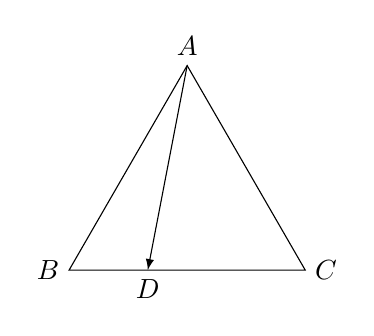
\begin{tikzpicture}[>=latex]
        \draw (0,0) node [left] {$B$} -- (3,0) node [right] {$C$} -- (1.5,{1.5*sqrt(3)}) node [above] {$A$} coordinate (A) -- cycle;
        \draw [->] (A) -- (1,0) node [below] {$D$};
    \end{tikzpicture}
\end{center}
\item 定义在$\mathbf{R}$上的偶函数$y=f(x)$, 当$x\ge 0$时, $f(x)=\lg (x^2-3x+3)$, 则$f(x)$在$\mathbf{R}$上的零点个数为\blank{50}个.
\item 将$6$辆不同的小汽车和$2$辆不同的卡车驶入如图所示的$10$个车位中的某$8$个内, 其中$2$辆卡车必须停在$A$与$B$的位置, 那么不同的停车位置安排共有\blank{50}种(结果用数值表示).
\begin{center}
    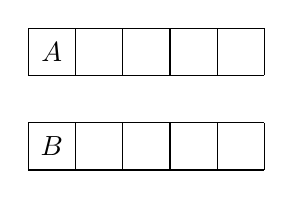
\begin{tikzpicture}[>=latex]
        \draw (0,0) node {$B$};
        \draw (0,1.2) node {$A$};
        \foreach \i in {-0.3,0.3,0.9,1.5}{\draw (-0.3,\i) -- (2.7,\i);};
        \foreach \i in {-0.3,0.3,...,2.8}{\draw (\i,-0.3) -- (\i, 0.3) (\i, 0.9) -- (\i, 1.5);};
    \end{tikzpicture}
\end{center}

% 赋能3 

\item 设集合$A=\{x||x-2|<1,x\in \mathbf{R}\}$, 集合$B=\mathbf{Z}$, 则$A\cap B=$\blank{50}.
\item 函数$y=\sin (\omega x-\dfrac{\pi}{3})$($\omega >0$)的最小正周期是$\pi$, 则$\omega =$\blank{50}.
\item 设$\mathrm{i}$为虚数单位, 在复平面上, 复数$\dfrac{3}{(2-\mathrm{i})^2}$对应的点到原点的距离为\blank{50}.
\item 若函数$f(x)=\log_2 (x+1)+a$的反函数的图像经过点$(4,1)$, 则实数$a=$\blank{50}.
\item 已知$(a+3b)^n$的展开式中, 各项系数的和与各项二项式系数的和之比为$64$, 则$n=$\blank{50}.
\item 甲、乙两人从$5$门不同的选修课中各选修$2$门, 则甲、乙所选的课程中恰有$1$门相同的选法有\blank{50}种.
\item 若圆锥的侧面展开图是半径为2$\text{cm}$, 圆心角为$270^\circ$的扇形, 则这个圆锥的体积为\blank{50}$\text{cm}^3$.
\item 若数列$\{a_n\}$的所有项都是正数, 且$\sqrt{a_1}+\sqrt{a_2}+\cdots +\sqrt{a_n}=n^2+3n$($n\in \mathbf{N}^*$), 则$\displaystyle\lim_{n\to\infty}\dfrac{1}{n^2}(\dfrac{a_1}{2}+\dfrac{a_2}{3}+\cdots +\dfrac{a_n}{n+1})=$\blank{50}.
\item 如图, 在$\triangle ABC$中, $\angle B=45^\circ$, $D$是$BC$边上的一点, $AD=5$, $AC=7$, $DC=3$, 则$AB$的长为\blank{50}.
\begin{center}
    \begin{tikzpicture}[scale = 0.5]
        \draw  (-6.830127018922193,0.)-- (3.,0.) node [below right] {$C$};
        \draw  (3.,0.)-- (-2.5,4.330127018922193) node [above] {$A$};
        \draw  (-2.5,4.330127018922193)-- (-6.830127018922193,0.) node [below left] {$B$};
        \draw  (-2.5,4.330127018922193)-- (0.,0.) node [below] {$D$};
    \end{tikzpicture}
\end{center}
\item 有以下命题:\\
\textcircled{1} 若函数$f(x)$既是奇函数又是偶函数, 则$f(x)$的值域为$\{0\}$; \\
\textcircled{2} 若函数$f(x)$是偶函数, 则$f(|x|)=f(x)$;\\
\textcircled{3} 若函数$f(x)$在其定义域内不是单调函数, 则$f(x)$不存在反函数;\\
\textcircled{4} 若函数$f(x)$存在反函数${{f}^{-1}}(x)$, 且${{f}^{-1}}(x)$与$f(x)$不完全相同, 则$f(x)$与${{f}^{-1}}(x)$图像的公共点必在直线$y=x$上; \\
其中真命题的序号是\blank{50}(写出所有真命题的序号).

% 赋能4

\item 若集合$A=\{x|y^2=x,y\in \mathbf{R}\}$, $B=\{y|y=\sin x,x\in \mathbf{R}\}$, 则$A\cap B=$\blank{50}.
\item 若$-\dfrac{\pi}{2}<\alpha <\dfrac{\pi}{2}$, $\sin \alpha =\dfrac{3}{5}$, 则$\cot 2\alpha =$\blank{50}.
\item 函数$f(x)=1+\log_2 x$($x\ge 1$)的反函数$f^{-1}(x)=$\blank{50}.
\item 若$(1+x)^5=a_0+a_1x+a_2x^2+\cdots+a_5x^5$, 则$a_1+a_2+\cdots+a_5=$\blank{50}.
\item 设$k\in \mathbf{R}$, $\dfrac{y^2}{k}-\dfrac{x^2}{k-2}=1$表示焦点在$y$轴上的双曲线, 则半焦距的取值范围是\blank{50}.
\item 设$m\in \mathbf{R}$, 若$f(x)=(m+1)x^{\tfrac{2}{3}}+mx+1$是偶函数, 则$f(x)$的单调递增区间是\blank{50}.
\item 方程$\log_2(9^x-5)=2+\log_2(3^x-2)$的解$x=$\blank{50}.
\item 已知圆$C:x^2+y^2+2kx+2y+k^2=0$($k\in \mathbf{R}$)和定点$P(1,-1)$, 若过$P$可以作两条直线与圆$C$相切, 则$k$的取值范围是\blank{50}.
\item 如图, 在直三棱柱$ABC-A_1B_1C_1$中, $\angle ABC=90^\circ$, $AB=BC=1$, 若$A_1C$与平面$B_1BCC_1$所成的角为$\dfrac{\pi}{6}$, 则三棱锥$A_1-ABC$的体积为\blank{50}.
\begin{center}
    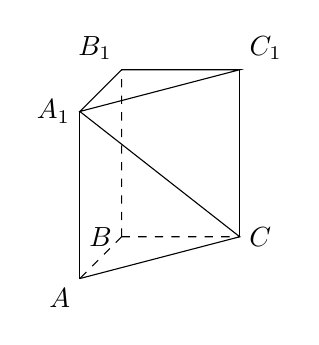
\begin{tikzpicture}[scale = 1.5]
        \draw [dashed] (0,0) -- (1,0) node [right] {$C$} coordinate (C) (0,0) -- (225:0.5) node [below left] {$A$} coordinate (A) (0,0) node [left] {$B$} coordinate (B) -- (0,{sqrt(2)}) node [above left] {$B_1$} coordinate (B1);
        \draw (A) --+ (0,{sqrt(2)}) node [left] {$A_1$} coordinate (A1);
        \draw (C) --+ (0,{sqrt(2)}) node [above right] {$C_1$} coordinate (C1);
        \draw (A1) -- (B1) -- (C1) -- (A1) -- (C) -- (A);
    \end{tikzpicture}
\end{center}
\item 设地球半径为$R$, 若$A$、$B$两地均位于北纬$45^\circ$, 且两地所在纬度圈上的弧长为$\dfrac{\sqrt{2}}{4}\pi R$, 则$A$、$B$之间的球面距离是\blank{50}(结果用含有$R$的代数式表示).

% 赋能5

\item 复数$\mathrm{i}(2+\mathrm{i})$的虚部为\blank{50}.
\item 设函数$f(x)=\begin{cases}\log_2 x, & x>0, \\ 4^x, & x\le 0,\end{cases}$ 则$f(f(-1))=$\blank{50}.
\item 已知$M=\{x||x-1|\le 2,x\in \mathbf{R}\}$, $P=\{x|\dfrac{1-x}{x+2}\ge 0,x\in \mathbf{R}\}$, 则$M\cap P=$\blank{50}.
\item 抛物线$y=x^2$上一点$M$到焦点的距离为$1$, 则点$M$的纵坐标为\blank{50}.
\item 已知无穷数列$\{a_n\}$满足$a_{n+1}=\dfrac12{a_n}$($n\in \mathbf{N}^*$), 且$a_2=1$, 记$S_n$为数列$\{a_n\}$的前$n$项和, 则$\displaystyle\lim_{n\to \infty}S_n=$\blank{50}.
\item 已知$x,y\in \mathbf{R}^+$, 且$x+2y=1$, 则$xy$的最大值为\blank{50}.
\item 已知圆锥的母线$l=10$, 母线与旋转轴的夹角$\alpha =30^\circ$, 则圆锥的表面积为\blank{50}.
\item 若$(2x^2+\dfrac1x)^n$($n\in \mathbf{N}^*$)的二项展开式中的第$9$项是常数项, 则$n=$\blank{50}.
\item 已知$A,B$分别是函数$f(x)=2\sin \omega x$($\omega >0$)在$y$轴右侧图像上的第一个最高点和第一个最低点, 且$\angle AOB=\dfrac\pi 2$, 则该函数的最小正周期是\blank{50}.
\item 将序号分别为1、2、3、4、5的$5$张参观券全部分给$4$人, 每人至少一张, 如果分给同一人的$2$张参观券连号, 那么不同的分法种数是\blank{50}.

% 赋能6

\item $\displaystyle\lim_{n\to\infty}\dfrac{2n+3}{n+1}=$\blank{50}.
\item 设全集$U=\mathbf{R}$, 集合$A=\{-1,0,1,2,3\}$, $B=\{x|x\ge 2\}$, 则$A\cap {\complement_U}B=$\blank{50}.
\item 不等式$\dfrac{x+1}{x+2}<0$的解集为\blank{50}.
\item 椭圆$\begin{cases} x=5\cos \theta,  \\ y=4\sin \theta  \end{cases}$($\theta$为参数)的焦距为\blank{50}.
\item 若函数$y=\begin{vmatrix}   \cos x & \sin x  \\   \sin x & \cos x  \\ \end{vmatrix}$的最小正周期为$a\pi $, 则实数$a$的值为\blank{50}.
\item 若点$(8,4)$在函数$f(x)=1+\log_a x$图像上, 则$f(x)$的反函数为\blank{50}.
\item 已知向量$\overrightarrow{a}=(1,2)$, $\overrightarrow{b}=(0,3)$, 则$\overrightarrow{b}$在$\overrightarrow{a}$的方向上的投影为\blank{50}.
\item 已知一个底面置于水平面上的圆锥, 其左视图是边长为6的正三角形, 则该圆锥的侧面积为\blank{50}.
\item 某班级要从$5$名男生和$2$名女生中选出$3$人参加公益活动, 则在选出的$3$人中男、女生
均有的概率为\blank{50}(结果用最简分数表示).
\item 设常数$a>0$, 若$(x+\dfrac ax)^9$的二项展开式中$x^5$的系数为$144$, 则$a=$\blank{50}.

% 赋能7

\item 设集合$M=\{x|x^2=x\}$, $N=\{x|\lg x\le 0\}$, 则$M\cap N=$\blank{50}.
\item 已知$a$、$b\in \mathbf{R}$, $\mathrm{i}$是虚数单位, 若$a+\mathrm{i}=2-b\mathrm{i}$, 则$(a+b\mathrm{i})^2=$\blank{50}.
\item 已知函数$f(x)=a^x-1$的图像经过$(1,1)$点, 则$f^{-1}(3)=$\blank{50}.
\item 不等式$x|x-1|>0$的解集为\blank{50}.
\item 已知$\overrightarrow a=(\sin x,\cos x)$, $\overrightarrow b=(\sin x,\sin x)$, 则函数$f(x)=\overrightarrow a\cdot \overrightarrow b$的最小正周期为\blank{50}.
\item 里约奥运会游泳小组赛采用抽签方法决定运动员比赛的泳道, 在由$2$名中国运动员和$6$名外国运动员组成的小组中, $2$名中国运动员恰好抽在相邻泳道的概率为\blank{50}.
\item 如图, 在棱长为$1$的正方体$ABCD-A_1B_1C_1D_1$中, 点$P$在截面$A_1DB$上, 则线段$AP$的最小值为\blank{50}.
\begin{center}
    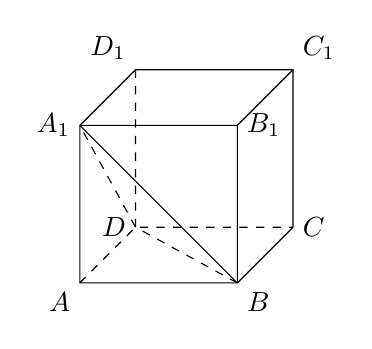
\begin{tikzpicture}
        \draw (0,0) node [below left] {$A$} coordinate (A) --++ (2,0) node [below right] {$B$} coordinate (B) --++ (45:{2/2}) node [right] {$C$} coordinate (C)
        --++ (0,2) node [above right] {$C_1$} coordinate (C1)
        --++ (-2,0) node [above left] {$D_1$} coordinate (D1) --++ (225:{2/2}) node [left] {$A_1$} coordinate (A1) -- cycle;
        \draw (A) ++ (2,2) node [right] {$B_1$} coordinate (B1) -- (B) (B1) --++ (45:{2/2}) (B1) --++ (-2,0);
        \draw [dashed] (A) --++ (45:{2/2}) node [left] {$D$} coordinate (D) --++ (2,0) (D) --++ (0,2);
        \draw (A1) -- (B);
        \draw [dashed] (B) -- (D) -- (A1);
    \end{tikzpicture}
\end{center}
\item 设$(1+x)^n=a_0+a_1x+a_2x^2+a_3x^3+\cdots +a_nx^n$, 若$\dfrac{a_2}{a_3}=\dfrac13$, 则$n=$\blank{50}.
\item 已知圆锥底面半径与球的半径都是$1\text{cm}$, 如果圆锥的体积与球的体积恰好也相等, 那么这个圆锥的侧面积是\blank{50}$\text{cm}^2$.
\item 设$P(x,y)$是曲线$C:\sqrt{\dfrac{x^2}{25}}+\sqrt{\dfrac{y^2}9}=1$上的点, $F_1(-4,0)$, $F_2(4,0)$, 则$|PF_1|+|PF_2|$的最大值为\blank{50}.

% 赋能8

\item 已知复数$z=2+\mathrm{i}$($\mathrm{i}$为虚数单位), 则$\overline{{z^2}}=$\blank{50}.
\item 已知集合$A=\{x|\dfrac12\le {2^x}<16\}$, $B=\{x|y=\log _2(9-x^2)\}$, 则$A\cap B=$\blank{50}。
\item 在二项式$(x+\dfrac2x)^6$的展开式中, 常数项是\blank{50}.
\item 等轴双曲线$x^2-y^2=a^2$与抛物线$y^2=16x$的准线交于$A$、$B$两点, 且$|AB|=4\sqrt3$, 则该双曲线的实轴长等于\blank{50}.
\item 若由矩阵$\begin{pmatrix}a & 2 \\ 2 & a\end{pmatrix}\begin{pmatrix}x \\ y\end{pmatrix}=\begin{pmatrix}a+2 \\ 2a\end{pmatrix}$表示$x$、$y$的二元一次方程组无解, 则实数$a=$\blank{50}.
\item 已知$f(x)=\sin\dfrac\pi 3x$, $A=\{1,2,3,4,5,6,7,8\}$, 现从集合$A$中任取两个不同元素$s$、$t$, 则使得$f(s)\cdot f(t)=0$发生的概率是\blank{50}.
\item 若圆锥侧面积为$20\pi$, 且母线与底面所成角为$\arccos \dfrac45$, 则该圆锥的体积为\blank{50}.
\item 已知数列$\{a_n\}$的通项公式为$a_n=n^2+bn$, 若数列$\{a_n\}$是单调递增数列, 则实数$b$的取值范围是\blank{50}.
\item 将边长为$10$的正三角形$ABC$, 按``斜二测''画法在水平放置的平面上画出为$\triangle A'B'C'$, 则$\triangle A'B'C'$中最短边的边长为\blank{50}(精确到0.01).
\item 已知点$A$是圆$O: x^2+y^2=4$上的一个定点, 点$B$是圆$O$上的一个动点, 若满足$|\overrightarrow{AO}+\overrightarrow{BO}|=|\overrightarrow{AO}-\overrightarrow{BO}|$, 则$\overrightarrow{AO}\cdot \overrightarrow{AB}=$\blank{50}.


\end{enumerate}

\end{document}